\documentclass[tikz,border=5mm]{standalone}
\usetikzlibrary{positioning,arrows.meta}

\begin{document}
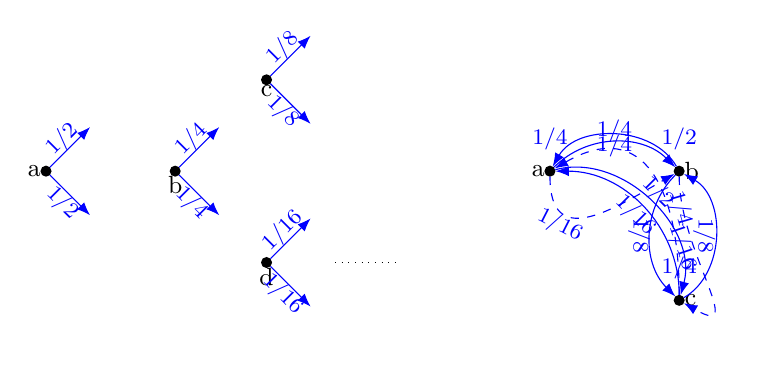
\begin{tikzpicture}[
    node distance=1.5cm,
    every node/.style={inner sep=0, outer sep=0},
    >=Latex,
    scale=0.8, % Adjust overall scaling for better fit
]

% Left diagram: Infinite Decision Tree
\node[circle,fill=black,minimum size=4pt,label=left:{\small a}] (A1) {};
\node[circle,fill=black,minimum size=4pt,right=of A1,label=below:{\small b}] (B1) {};
\node[circle,fill=black,minimum size=4pt,above right=of B1,label=below:{\small c}] (C1) {};
\node[circle,fill=black,minimum size=4pt,below right=of B1,label=below:{\small d}] (D1) {};

% Edges with labels
\draw[blue,->] (A1) -- ++(0.7,0.7) node[midway,above,sloped] {\footnotesize $1/2$};
\draw[blue,->] (A1) -- ++(0.7,-0.7) node[midway,below,sloped] {\footnotesize $1/2$};

\draw[blue,->] (B1) -- ++(0.7,0.7) node[midway,above,sloped] {\footnotesize $1/4$};
\draw[blue,->] (B1) -- ++(0.7,-0.7) node[midway,below,sloped] {\footnotesize $1/4$};

\draw[blue,->] (C1) -- ++(0.7,0.7) node[midway,above,sloped] {\footnotesize $1/8$};
\draw[blue,->] (C1) -- ++(0.7,-0.7) node[midway,below,sloped] {\footnotesize $1/8$};

\draw[blue,->] (D1) -- ++(0.7,0.7) node[midway,above,sloped] {\footnotesize $1/16$};
\draw[blue,->] (D1) -- ++(0.7,-0.7) node[midway,below,sloped] {\footnotesize $1/16$};

% Add dotted line to indicate continuation
\draw[dotted] ([xshift=1cm]D1.east) -- ++(1cm,0);

% Right diagram: Balancer Embedding
\node[circle,fill=black,minimum size=4pt,label=left:{\small a}] (A2) at (8,0) {};
\node[circle,fill=black,minimum size=4pt,right=of A2,label=right:{\small b}] (B2) {};
\node[circle,fill=black,minimum size=4pt,below=of B2,label=right:{\small c}] (C2) {};

% Paths for the decision tree
\path[blue,->]
    (A2) edge[bend left=45] node[midway,above,sloped] {\footnotesize $1/4$} (B2)
    (A2) edge[bend left=60] node[midway,above,sloped] {\footnotesize $1/2$} (C2)
    (B2) edge[bend right=45] node[midway,below,sloped] {\footnotesize $1/8$} (C2)
    (B2) edge[bend right=60] node[midway,below,sloped] {\footnotesize $1/4$} (A2)
    (C2) edge[bend right=45] node[midway,below,sloped] {\footnotesize $1/16$} (A2)
    (C2) edge[bend right=60] node[midway,below,sloped] {\footnotesize $1/8$} (B2);

% Additional arcs for balancing
\draw[blue,->,dashed]
    (A2) to[out=-90,in=-150,looseness=1.5] node[pos=0.3,below,sloped] {\footnotesize $1/16$} (B2);
\draw[blue,->,dashed]
    (B2) to[out=-90,in=-30,looseness=1.5] node[pos=0.3,below,sloped] {\footnotesize $1/16$} (C2);
\draw[blue,->,dashed]
    (C2) to[out=90,in=30,looseness=1.5] node[pos=0.3,above,sloped] {\footnotesize $1/4$} (A2);

% Annotations for probabilities
\node[blue,above=0.2cm of A2] {\footnotesize $1/4$};
\node[blue,above=0.2cm of B2] {\footnotesize $1/2$};
\node[blue,above=0.2cm of C2] {\footnotesize $1/4$};

\end{tikzpicture}
\end{document}